\usetikzlibrary{arrows.meta,calc,patterns}

\begin{frame}{split caches; multiple cores}
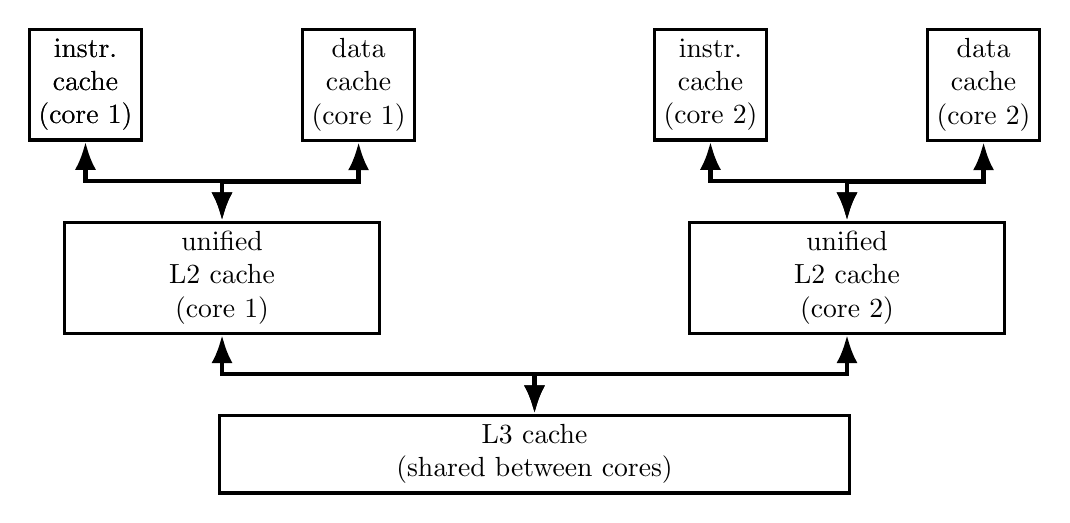
\begin{tikzpicture}
    \tikzset{
        >=Latex,
        connect/.style={<->,ultra thick},
        cache/.style={draw,very thick,align=center},
    }
\node[cache] (icache1) {instr. \\ cache \\ (core 1)};
\node[cache,anchor=west] (dcache1) at ([xshift=2cm]icache1.east) {data \\ cache \\ (core 1)};
\node[cache] (icache2) {instr. \\ cache \\ (core 1)};
\node[cache,anchor=west] (icache2) at ([xshift=3cm]dcache1.east) {instr. \\ cache \\ (core 2)};
\node[cache,anchor=west] (dcache2) at ([xshift=2cm]icache2.east) {data \\ cache \\ (core 2)};
\node[cache, minimum width=4cm,anchor=north] (l21) at ([yshift=-1cm]$(icache1.south)!0.5!(dcache1.south)$) {unified \\ L2 cache \\ (core 1)};
\node[cache, minimum width=4cm,anchor=north] (l22) at ([yshift=-1cm]$(icache2.south)!0.5!(dcache2.south)$) {unified \\ L2 cache \\ (core 2)};
    \node[cache, minimum width=8cm,anchor=north] (l3) at ([yshift=-1cm]$(l21.south)!0.5!(l22.south)$) {L3 cache \\ (shared between cores)};
\foreach \fromC/\toC in {icache1/l21,dcache1/l21,icache2/l22,dcache2/l22,l21/l3,l22/l3} {
\draw[connect] (\fromC.south) -- ++(-0cm,-.5cm) -| (\toC.north);
}
\end{tikzpicture}
\end{frame}

\begin{frame}{hierarchy and instruction/data caches}
    \begin{itemize}
    \item typically separate data and instruction caches for L1
    \vspace{.5cm}
    \item (almost) never going to read instructions as data or vice-versa
    \item avoids instructions evicting data and vice-versa
    \item can optimize instruction cache for different access pattern
    \item easier to build fast caches: that handles less accesses at a time
    \end{itemize}
\end{frame}

\begin{frame}{inclusive versus exclusive}
\begin{tikzpicture}
\tikzset{
    >=Latex,
    connect/.style={<->,ultra thick},
    cache/.style={draw,very thick},
    fill 1/.style={pattern color=blue!50!black,pattern=crosshatch},
    fill 2/.style={pattern color=orange,pattern=dots},
}
\node (l2 incl label) at (2.5, 6.5) {L2 inclusive of L1};
\node[font=\small,anchor=north,align=center] at (l2 incl label.south) {
    everything in L1 cache duplicated in L2 \\
    adding to L1 also adds to L2
};
\node[anchor=south]  at (1, 2) {L1 cache};
\node[anchor=south]  at (4, 4) {L2 cache};
\draw[cache] (0, 0) rectangle ++(2, 2);
\path[fill 1] (0, 0) rectangle ++(2, 2);
\path[fill 2] (3, -1.5) rectangle ++(2,1);
\path[fill 1] (3, -0.5) rectangle ++(2, .5);
\path[fill 2] (3, 0) rectangle ++(2,.25);
\path[fill 1] (3, 0.25) rectangle ++(2, .3);
\path[fill 2] (3, 0.55) rectangle ++(2,.65);
\path[fill 1] (3, 1.2) rectangle ++(2, .6);
\path[fill 2] (3, 1.8) rectangle ++(2,.2);
\path[fill 1] (3, 2) rectangle ++(2, .6);
\path[fill 2] (3, 2.6) rectangle ++(2,1.4);
\draw[cache] (3, -1.5) rectangle ++(2, 5.5);

\begin{scope}[xshift=8cm]
\node (l2 excl label) at (2.5, 6.5) {L2 exclusive of L1};
\node[font=\small,anchor=north,align=center] at (l2 excl label.south) {
    L2 contains different data than L1 \\
    adding to L1 must remove from L2 \\
    probably evicting from L1 adds to L2
};
\node[anchor=south]  at (1, 2) {L1 cache};
\node[anchor=south]  at (4, 4) {L2 cache};
\path[fill 1] (0, 0) rectangle ++(2, 2);
\draw[cache] (0, 0) rectangle ++(2, 2);
\draw[cache,fill 2] (3, -1.5) rectangle ++(2, 5.5);
\end{scope}
\begin{visibleenv}<2>
    \draw[overlay,red,very thick] (-1,-1.75) rectangle (6.25, 7);
    \fill[fill opacity=0.95,fill=white] (6.75, -1.75) rectangle (14, 7)
        node[midway,align=left,font=\small] {
            inclusive policy: \\
            no extra work on eviction \\
            but duplicated data \\
            ~ \\
            easier to explain when \\
            L$k$ shared by multiple L$(k-1)$ caches?
        };
\end{visibleenv}
\begin{visibleenv}<3>
    \draw[overlay,red,very thick] (6.75, -1.75) rectangle (14, 7);
    \fill[fill opacity=0.95,fill=white](-1,-1.75) rectangle (6.25, 7)
        node[midway,align=left,font=\small] {
            exclusive policy: \\
            avoid duplicated data \\
            sometimes called \textit{victim cache} \\
            (contains cache eviction victims) \\
            ~ \\
            makes less sense with multicore
        };
\end{visibleenv}
\end{tikzpicture}
\end{frame}

